\section{Theorie}
\label{sec:Theorie}

\subsection{Berechnung der Suszeptibilität aus atomaren Größen}
Die magnetische Suszeptibilität ist eine Größe, welche die Magnetisierbarkeit eines Materials in einem äußeren Feld angibt.
Man unterscheidet dabei zwischen der diamagnetischen und der paramagnetischen Suszeptibilität.
Die diamagnetische Suszeptibilität ist eine allgemeine Eigenschaft der Materie.
Hierbei wird durch ein externer Feld ein magnetisches Moment induziert.
Dies resultiert in einem eigenem Magnetfeld, welches dem äußeren entgegengesetzt ist.
Die Suszeptibilität ist somit negativ.
Für diesen Versuch wird hingegen die paramagnetische Suszeptibilität untersucht.
Sie tritt nur bei Atomen, Ionen oder Molekülen auf, die einen nichtverschwindenden Drehimpuls aufweisen.
Die paramagnetische Suszeptibilität ist von der Ausrichtung der Momente abhängig und dadurch stark Temperatur abhängig.
Der Gesamtdrehimpuls $\vec{J}$ eines Teilchens setzt sich dabei aus dem Bahndrehimpuls der Elektronenhülle, dem Spin der Elektronen und dem Kerndrehimpuls zusammen.
Für schwache äußere Felder kann der Gesamtdrehimpuls als lediglich aus dem Spin $\vec{S}$ und dem Bahndrehimpuls $\vec{L}$ zusammengesetzt verstanden werden.
Für diese lässt sich mittels der Quantenmechanik die Beträge der entsprechenden magnetischen Momente berechnen.
Hierbei sind lediglich die zu $\vec{J}$ parallelen, bzw. antiparallelen Komponenten der Momente messbar.
Die Winkelbeziehungen sind daher in Abbildung \ref{fig:Winkelbeziehungen} dargestellt.

\begin{figure}
  \centering
  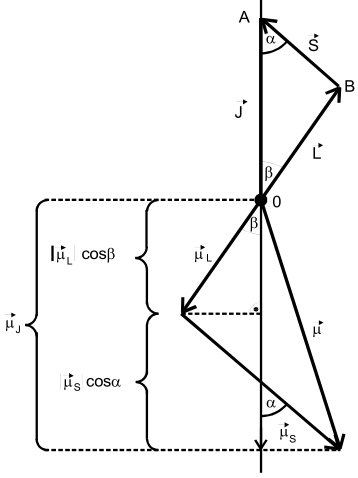
\includegraphics[width=0.5\textwidth]{images/Winkelbeziehungen.png}
  \caption{Darstellung der Vektoren der magnetischen Momente und deren Zusammenhänge zum Gesamtdrehimpuls, entnommen der Veruchsanleitung\cite[174]{sample}}
  \label{fig:Winkelbeziehungen}
\end{figure}

Hier muss irgendwann auch noch was zum Landefaktor hin.

Aus der quantenmechanischen Richtungsquantelung ergibt sich, dass der Winkel zwischen dem gesamten magnetischen Moment $\mu_J$ und dem äußeren magnetischen Feld nicht beliebig sein darf, sondern vielmehr ein ganzzahliges Vielfaches des Bohrschen Magnetons und dem gyromagnetischen Verhältnis sein muss.
Diese ganzzahlige Größe m wird auch die Orientierungsquantenzahl genannnt und ergibt sich aus dem Zeeman-Effekt.

\subsection{Berechnung der Suszeptibilität aus einer geeigneten Messanordnung}

Die Suszeptibilität kann durch die Änderung der Induktivität einer Spule innerhalb einer Brückenschaltung ermittelt werden.
Diese äußert sich durch die Änderung der gemessenen Brückenspannung der Brückenschaltung.
Die Änderung der Induktivität entsteht, wenn man in eine der Spulen, hier L$_M$ die entsprechende Probe einführt.
Die verwendete Schaltung ist in Abbildung \ref{fig:Brückenschaltung} dargestellt.

\begin{figure}
  \centering
  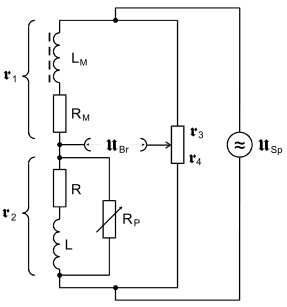
\includegraphics[width=0.5\textwidth]{images/Brueckenschaltung.png}
  \caption{Die für die Messung verwendete Brückenschaltung, entnommen der Versuchsanleitung\cite[179]{sample}}
  \label{fig:Brückenschaltung}
\end{figure}

Dabei ist der Widerstand R$_3$ und R$_4$ ein regelbarer Widerstand, der für beide Widerstände die gleichen Werte einstellt.
R$_1$ und R$_2$ stellen die Widerstände der Spulen dar.
R$_P$ kann für die Rechnungen vernachlässigt werden, allerdings ist er für die Eichung der Messapparatur von großer Bedeutung.
Berücksichtig man den Aufbau der Brückenschaltung, so kann man durch das Verhältnis der Brückenspannung vor und nach der Einführung der Probe in die Spule die Suszeptibilität nach der Gleichung:

\begin{equation}
  \Chi = 4 \frac{F}{Q} \frac{U_{Br}}{U_{Sp}}
\end{equation}

errechnen.
Dabei stellt F den Querschnitt der Spule, Q den Querschnitt der Probe, $U_{Br}$ die Brückenspannung nach und $U_{Sp}$ die Brückenspannung vor dem Einführen der Probe dar.
Diese Gleichung ist nur für hohe Frequenzen hinreichend genau.
Es ist hierbe drauf zu achten, dass die zwei genannten Brückenspannungen nur für abgeglichene Brückenschaltungen gelten.
Weiterhin ist darauf zu achten, dass es sich bei den verwendeten Proben um staubförmige Präparate handelt.
Diese lassen sich nicht auf die tatsächliche Dichte eines Einkristalls stopfen.
Der tatsächliche Queschnitt Q$_{real}$ weicht daher von dem theoretischen ab.
Es wird daher der Quotient zwischen der wahren Dichte eines Einkristalls $\rho_w$ und der der gestopften Probe $\rho_p$ gesucht.
Dieser gibt das Verhältnis des theoretischen und des tatsächlichen Querschnitts an.
Die Dichte der Probe wird dabei durch die folgende Relation bestimmt:

\begin{equation}
  \rho_p = \frac{M_p}{Q L}
\end{equation}

Der tatsächliche Querschnitt weist dann folgende Relation auf:

\begin{equation}
  Q_{real} = \frac{M_p}{L \rho_w}
\end{equation}

Die so entstehenden Brückenspannungen sind in der Größenordnung von Störspannungen.
Die Störspannungen müssen somit heraus gefiltert und die Brückenspannungen amplifiziert werden.
Dies kann hinreichend genau durch einen Selektivverstärker geschehen.
Dieser weist eine Filterkurve auf, die in ausreichender Genauigkeit die monofrequente Brückenspannung herausfiltert.
Eine beispielhafte Kruve ist in Abbildung \ref{fig:theofilterkurve} dargestellt.
U$_A$ bezeichnet dort die Ausgangs- und U$_E$ die Eingangsspannung.

\begin{figure}
  \centering
  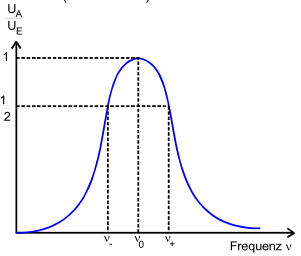
\includegraphics[width=0.5\textwidth]{images/theodiefilterkurve.png}
  \caption{Beispielhafte Filterkurve eines Selektivverstärkers, entnommen der Versuchsanleitung\cite[182]{sample}}
  \label{fig:theofilterkurve}
\end{figure}

Die Güte Q eines solchen Selektivverstärkers kann man dabei durch die größen $\nu_0$, $\nu_-$ und $\nu_+$ berechnet werden.
Es ergibt sich dafür folgende Gleichung:

\begin{equation}
  Q = \frac{\nu_0}{\nu_+ - \nu_-}
\end{equation}

Eine weitere Methode stellt die Bestimmung der Abgleichbedingung für R$_3$ und R$_4$ dar.
Hierbei kann durch die Änderung der Widerstände um die Abgleichbedingung zu erfüllen, die Suszeptibilität berechnet werden.
Dies erfolgt mittels dieser Gleichung:

\begin{equation}
  \Chi = 2 \frac{\Delta R}{R_3} \frac{F}{Q}
\end{equation}
